\documentclass{beamer}
\usepackage{graphicx}
\usepackage{xcolor}
\usepackage{tikz}

% 自定义颜色
\definecolor{purpleblue}{RGB}{80, 80, 180}
\definecolor{lightgray}{RGB}{230, 230, 230}
\definecolor{novelPurple}{RGB}{98, 54, 255} 
\definecolor{darkgray}{RGB}{50, 50, 50}

% 主题设置
\usetheme{Madrid}  
\usecolortheme{dolphin} 

% 设置字体（移除 fontspec，确保 pdfLaTeX 兼容）
\setbeamerfont{title}{size=\Large,series=\bfseries}
\setbeamerfont{frametitle}{size=\LARGE,series=\bfseries}
\setbeamercolor{frametitle}{fg=white, bg=novelPurple}
\setbeamercolor{title}{fg=white, bg=purpleblue}

% 封面信息
\title[SAT Hard Question]{\textbf{SAT Hard Question 10}}
\author{\textbf{Jack Zeng}}
\institute{\textcolor{white}{\textbf{Novel Prep}}}
\date{\today} 

\begin{document}

% --- Title Slide ---
\begin{frame}
    \titlepage
    \vfill
    \begin{flushright}
        \textcolor{purpleblue}{\Huge \textbf{Novel Prep}}
    \end{flushright}
\end{frame}


\begin{frame}
    \begin{tikzpicture}[remember picture, overlay]
        % 设置浅色渐变背景
        \shade[top color=softPurple, bottom color=softGray] 
            (current page.north west) rectangle (current page.south east);
        
        % 添加高斯模糊光晕
        \fill[white, opacity=0.3] (current page.center) circle (4cm);
        
        % 主标题
        \node[align=center] at (current page.center) {
            {\Huge\bfseries\textcolor{purpleblue}{Novel Prep}} \\[0.5cm]
            {\Large\itshape\textcolor{lightText}{Excellence in SAT Prep}}
        };

        % 添加柔和光点（点缀）
        \foreach \x in {1,2,3,4,5} {
            \fill[purpleblue, opacity=0.2] (rand*10-5, rand*7-3.5) circle (0.1+\x*0.05);
        }

        ;
    \end{tikzpicture}
\end{frame}



\begin{frame}{Parallel Lines and Transversals – Angles}
\small
In the figure, parallel lines $a$ and $b$ are intersected by lines $c$, $d$, and $e$.

If $z = 49^\circ$, $y = 136^\circ$, and $v < z$, which statement about $x$ and $w$ must be true?

\begin{center}
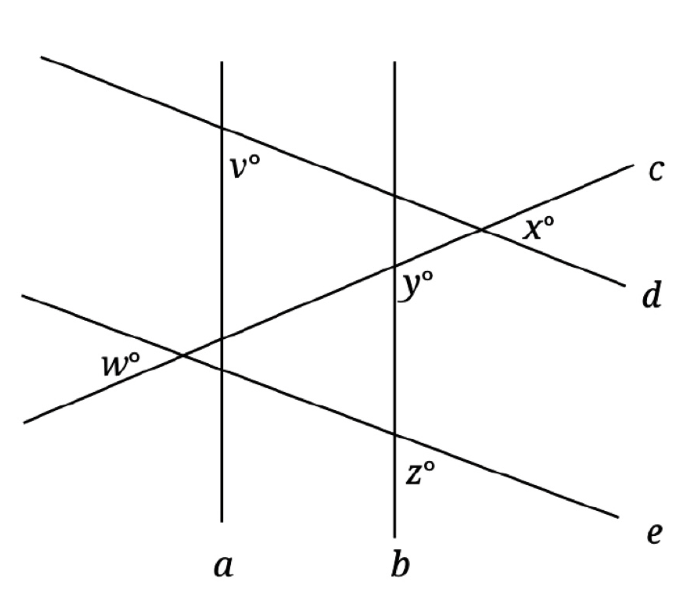
\includegraphics[width=0.4\textwidth]{f8.png}
\end{center}

\begin{enumerate}
    \item[A.] $x < w$
    \item[B.] $x > w$
    \item[C.] $x = w$
    \item[D.] $x + w = 90$
\end{enumerate}
\end{frame}

\begin{frame}{Solution: Parallel Lines and Angles}
\small
\textbf{Given:}
\begin{itemize}
    \item $z = 49^\circ$
    \item $y = 136^\circ$
    \item $v < z$
\end{itemize}

\textbf{Step 1: Solve for } $x$:
\[
x = 180^\circ - y = 180^\circ - 136^\circ = 44^\circ
\]

\textbf{Step 2: Understand the relation between } $v$ and $w$:
\begin{itemize}
    \item $w$ corresponds to $v$ via alternate interior angles
    \item Since $v < z = 49^\circ$, then $w < 49^\circ$
\end{itemize}

\textbf{Step 3: Compare:}
\[
x = 44^\circ,\quad w < 49^\circ \Rightarrow \boxed{x > w}
\]

\textbf{Correct Answer:} \boxed{\text{B. } x > w}
\end{frame}

\begin{frame}{Minimum Value of Exponential Functions}
\small
The functions $f$ and $g$ are defined by the given equations below, where $x \geq 0$.

Which of the following equations displays, as a constant or coefficient, the minimum value of the function it defines?

\begin{itemize}
    \item[I.] $f(x) = 16(1.3)^{x+5}$
    \item[II.] $g(x) = 16(1.09)(1.3)^{x+3} $
\end{itemize}

\begin{enumerate}
    \item[A.] I only
    \item[B.] II only
    \item[C.] I and II
    \item[D.] Neither I nor II
\end{enumerate}
\end{frame}


\begin{frame}{Solution: Minimum Value as Constant or Coefficient}
\footnotesize

\textbf{Function I:} $f(x) = 16(1.3)^{x + 5}$
\begin{itemize}
    \item Since $1.3 > 1$, the exponential function increases as $x$ increases.
    \item So $f(x)$ is an increasing function.
    \item The minimum value occurs at $x = 0$:
    \[
    f(0) = 16(1.3)^5 \approx 16(3.7129) \approx 59.41
    \]
    \item The minimum value is not 16, and 16 is not the minimum value of $f(x)$.
\end{itemize}

\vspace{0.1cm}
\textbf{Function II:} $g(x) = 16(1.09)(1.3)^{x + 3}$
\begin{itemize}
    \item $(1.3)^{x + 3}$ increases as $x$ increases, and $1.09$ is a constant.
    \item So $g(x)$ is also increasing.
    \item The minimum value occurs at $x = 0$:
    \[
    g(0) = 16(1.09)(1.3)^3 \approx 16(1.09)(2.197) \approx 38.41
    \]
    \item Again, 16 is not the minimum value, and is not part of the output.
\end{itemize}

\vspace{0.1cm}
\textbf{Conclusion:} Neither function displays its minimum value as a constant or coefficient.

\textbf{Correct Answer:} \boxed{\text{D. Neither I nor II}}

\end{frame}



\begin{frame}{Y-intercept of a Rational Function}
\small
The table shows values of $x$ and corresponding values of $g(x)$, where:

\[
g(x) = \frac{f(x)}{x + 3}
\quad \text{and} \quad f(x) \text{ is a linear function}
\]

What is the $y$-intercept of the graph of $y = f(x)$ in the $xy$-plane?

\begin{center}
\begin{tabular}{|c|c|}
\hline
$x$ & $g(x)$ \\
\hline
$-15$ & $3$ \\
$-6$ & $0$ \\
$9$ & $5$ \\
\hline
\end{tabular}
\end{center}

\begin{enumerate}
    \item[A.] (0, $-6$)
    \item[B.] (0, $4$)
    \item[C.] (0, $8$)
    \item[D.] (0, $24$)
\end{enumerate}
\end{frame}

\begin{frame}{Solution: Finding the Y-intercept of $f(x)$}
\small

\textbf{Step 1: Use the formula:}
\[
g(x) = \frac{f(x)}{x + 3} \Rightarrow f(x) = g(x)(x + 3)
\]

\textbf{Step 2: Calculate $f(x)$ values:}
\begin{itemize}
    \item At $x = -15$, $f(x) = 3(-15 + 3) = 3(-12) = -36$
    \item At $x = -6$, $f(x) = 0(-6 + 3) = 0$
    \item At $x = 9$, $f(x) = 5(9 + 3) = 5(12) = 60$
\end{itemize}

\textbf{Step 3: Use two points to find the line $f(x)$:}
\begin{itemize}
    \item Points: $(-6, 0)$ and $(9, 60)$
    \item Slope $m = \frac{60 - 0}{9 - (-6)} = \frac{60}{15} = 4$
    \item Line: $f(x) = 4x + b$, plug in $(-6, 0)$:
    \[
    0 = 4(-6) + b \Rightarrow b = 24
    \]
\end{itemize}

\textbf{Y-intercept:} $(0, 24)$

\textbf{Correct Answer:} \boxed{\text{D. (0, 24)}}
\end{frame}

\begin{frame}{Percent Problem – Variables and Percentages}
\small
The positive number $a$ is $2106\%$ of the sum of the positive numbers $b$ and $c$, and $b$ is $81\%$ of $c$.

What percent of $b$ is $a$?

\begin{enumerate}
    \item[A.] $4706\%$
    \item[B.] $2600\%$
    \item[C.] $38.12\%$
    \item[D.] $21.87\%$
\end{enumerate}
\end{frame}

\begin{frame}{Solution: Percent Relationship}
\small
\textbf{Step 1: Express $b$ in terms of $c$:}
\[
b = 0.81c
\]

\textbf{Step 2: Use the information that $a$ is $2106\%$ of the sum of $b + c$:}
\[
a = 2106\% \cdot (b + c) = 21.06 \cdot (0.81c + c) = 21.06 \cdot 1.81c = 38.065c
\]

\textbf{Step 3: What percent of $b$ is $a$?}
\[
\frac{a}{b} = \frac{38.065c}{0.81c} = \frac{38.065}{0.81} \approx 47.006 = 4706\%
\]

\textbf{Correct Answer:} \boxed{\text{A. } 4706\%}
\end{frame}



\begin{frame}{Polynomial Roots – Sum of Roots}
\small
In the given equation, $u$ is a positive constant. The sum of the solutions to the equation is 1. What is the value of $u$?

\[
7x^2(3x - 11)(3x - u) = 0
\]

\begin{enumerate}
    \item[A.] $1$
    \item[B.] $-8$
    \item[C.] $\dfrac{11}{3}$
    \item[D.] $\dfrac{8}{3}$
\end{enumerate}
\end{frame}

\begin{frame}{Solution: Sum of Solutions}
\small
\textbf{Step 1: Identify the roots from the factored form:}
\[
7x^2(3x - 11)(3x - u) = 0
\Rightarrow x = 0 \text{ (double root), } \frac{11}{3}, \frac{u}{3}
\]

\textbf{Step 2: Use sum of all roots:}
\[
0 + 0 + \frac{11}{3} + \frac{u}{3} = 1
\Rightarrow \frac{11 + u}{3} = 1
\Rightarrow 11 + u = 3
\Rightarrow u = 1 - 11 = -8
\]


\end{frame}


\begin{frame}{Solving a Quadratic Equation}
\small
Which of the following values of $x$ satisfy the equation
\[
-3x^2 + 12x + 4 = 0 ?
\]

\begin{enumerate}
    \item[A.] $0$
    \item[B.] $-2$ and $2$
    \item[C.] $2 - \dfrac{2\sqrt{6}}{3}$ and $2 + \dfrac{2\sqrt{6}}{3}$
    \item[D.] $2 - \dfrac{4\sqrt{3}}{3}$ and $2 + \dfrac{4\sqrt{3}}{3}$
\end{enumerate}
\end{frame}

\begin{frame}{Solution: Solving a Quadratic Equation}
\small
\textbf{Step 1: Identify coefficients.}
\begin{itemize}
    \item $a = -3$, $b = 12$, $c = 4$
\end{itemize}

\textbf{Step 2: Use the quadratic formula.}
\[
x = \frac{-b \pm \sqrt{b^2 - 4ac}}{2a}
\]

\textbf{Step 3: Compute discriminant.}
\[
\Delta = b^2 - 4ac = 144 + 48 = 192 = 64 \cdot 3
\Rightarrow \sqrt{192} = 8\sqrt{3}
\]

\textbf{Step 4: Solve for roots.}
\[
x = \frac{-12 \pm 8\sqrt{3}}{-6}
= 2 \pm \frac{4\sqrt{3}}{3}
\]

\textbf{Correct Answer:} \boxed{\text{D}}
\end{frame}



\begin{frame}{Angles Formed by Parallel Lines}
\small
A line intersects two parallel lines, forming four acute angles and four obtuse angles. The measure of one of these eight angles is $(7x - 250)^\circ$. The sum of the measures of four of the eight angles is $k$.

Which of the following could \textbf{not} be equivalent to $k$ for all values of $x$?

\begin{enumerate}
    \item[A.] $-14x + 1540$
    \item[B.] $14x - 320$
    \item[C.] $-28x + 1720$
    \item[D.] $360$
\end{enumerate}
\end{frame}

\begin{frame}{Solution: Parallel Line Angle Sums}
\small

\[
\boxed{\text{A is not equivalent to } k}
\]
\end{frame}


\begin{frame}{\textbf{Triangle Inequality Theorem}}
The triangle inequality theorem states that the sum of any two sides of a triangle must be greater than the length of the third side.

If a triangle has side lengths of $7$ and $10$, which inequality represents the possible lengths, $x$, of the third side of the triangle?

\begin{itemize}
    \item[A.] $x < 17$
    \item[B.] $x > 17$
    \item[C.] $3 < x < 17$
    \item[D.] $x < 3$ or $x > 17$
\end{itemize}
\end{frame}


\begin{frame}{\textbf{Solution to Triangle Inequality Problem}}
Let the three sides be $7$, $10$, and $x$. Apply the triangle inequality:

\begin{align*}
x + 7 &> 10 \quad \Rightarrow \quad x > 3 \\
x + 10 &> 7 \quad \Rightarrow \quad x > -3 \quad \text{(always true since } x > 3) \\
7 + 10 &> x \quad \Rightarrow \quad x < 17
\end{align*}

Combining the valid inequalities:
\[
3 < x < 17
\]

\textbf{Correct Answer: C. } $3 < x < 17$
\end{frame}





\end{document}